\begin{figure}[H]
\centering
\resizebox{0.9\textwidth}{!}{%
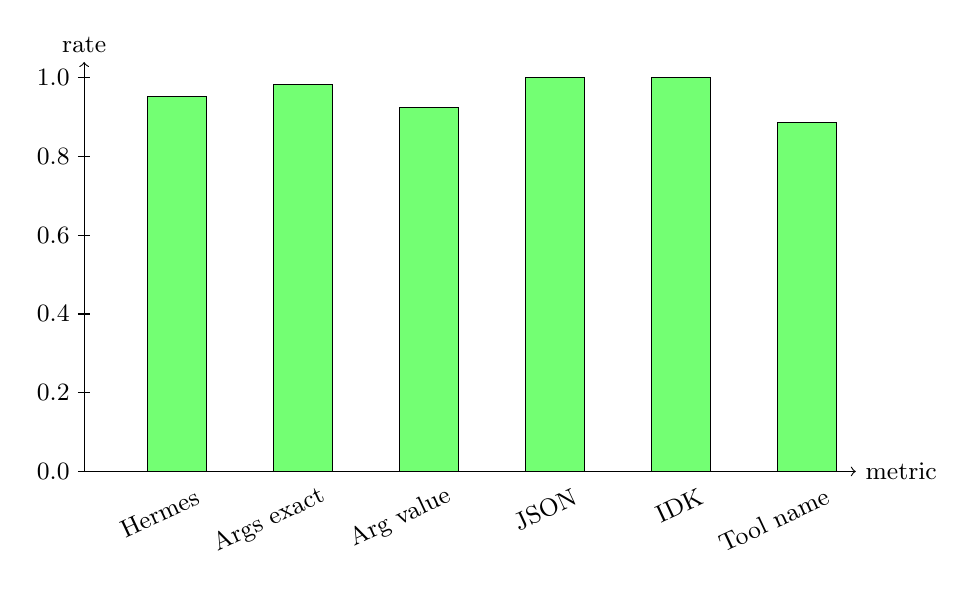
\begin{tikzpicture}[font=\small]
  \draw[->] (0,0) -- (9.8,0) node[right]{metric};
  \draw[->] (0,0) -- (0,5.2) node[above]{rate};
  \foreach \y/\lab in {0/0.0,1/0.2,2/0.4,3/0.6,4/0.8,5/1.0}
    {\draw (-0.08,\y) -- (0.08,\y) node[left=4pt]{\lab};}
  \foreach \x/\name/\val in {
    0.8/Hermes/4.76,
    2.4/Args exact/4.91,
    4.0/Arg value/4.62,
    5.6/JSON/5.00,
    7.2/IDK/5.00,
    8.8/Tool name/4.43
  }{
    \draw[fill=green!55] (\x,0) rectangle ++(0.75,\val);
    \node[rotate=25, anchor=east] at (\x+0.75,-0.25) {\name};
  }
\end{tikzpicture}%
}
\caption{Decoupled interface metrics on 242 held-out prompts. Tool-name exact copying is the remaining boundary; schema-grounded calls, exact arguments, JSON, and IDK pass.}
\label{fig:interface_metrics}
\end{figure}

